%\usepackage{multirow}
%\usepackage{amsmath}
%\usepackage[english]{babel}
%\usepackage{algorithm}
%\usepackage{algpseudocode}
%\usepackage{graphicx}
%\usepackage[T1]{fontenc}
%\usepackage{tikz}
%\usepackage{flushend}
%\usepackage[caption=false,font=footnotesize]{subfig}
%\usepackage{url}
%\usepackage{cite}

%\usepackage{listings}
%\lstset{
%  language=C++,
%  basicstyle=\footnotesize\ttfamily,
%}
%\lstset{aboveskip=-5pt,belowskip=-10pt}


\chapter{Semi-Static and Dynamic Load Balancing for Asynchronous Hurricane Storm Surge Simulations}

% \listoftoddos

\section{Introduction}
% why hurricane simulations are important
%Hurricane events are incredibly deadly and costly natural disasters.
Since 1980, seven out of the ten most costly US climate disasters were hurricanes, with Hurricane Katrina being the most expensive\cite{noaa}. Hurricanes Harvey, Maria, and Irma, which occurred in 2017, are expected to be among the five most costly US natural disasters.
The utilization of computational models can provide local officials with high fidelity tools to assist in evacuation efforts and mitigate loss of life and property.
%why we need HPC
Due to the highly nonlinear nature of hurricane dynamics and stringent time constraints, high performance computing (HPC) plays a cornerstone role in providing accurate predictions of flooding.
Because of the importance of fast, efficient models, there is a significant interest in improving the speed and quality of these computational tools.

%how computing is changing
Even as the speed of supercomputers is drastically increasing, the end of Moore's law and the introduction of many-core architectures represent a tectonic shift in the HPC community.
In particular, the degree of hardware parallelism is increasing at an exponential rate and the cost of data movement and synchronization is increasing faster than the cost of computation~\cite{KoggeCiSE2014}.
% , and hardware is becoming increasingly irregular due to the use of accelerators and susceptibility to failure.
% In order to achieve good resource utilization on these machines, task-based programming and execution models are being developed to
As a result, asynchronous task-based programming has been of great interest due to its potential to express increased software parallelism, introduce more flexible load balancing capabilities, and hide the cost of communication through task over-decomposition ~\cite{charm,hpx,legion,ocr,parsec,starpu,uintah,darma}.
%Examples of major task-based programming and execution models include Charm++, HPX~\cite{hpx}, Legion~\cite{legion}, OCR~\cite{ocr}, PaRSEC~\cite{parsec}, StarPU~\cite{starpu}, etc.
%There are also domain-specific task-based programming systems, such as the Uintah AMR Framework~\cite{uintah}, and task-based portability layers such as DARMA~\cite{darma}.
% Additionally, task-based execution may help address issues such as hardware fault tolerance.
These programming models decouple the specification of the algorithm from the task scheduling mechanism, which determines where and when each task may execute and orchestrates the movement of required data between the tasks.
Furthermore, lightweight, one-sided messaging protocols that support active messages have the potential to reduce the overheads associated with inter-process communication and synchronization, which will become even more important as parallelism increases.
However, transitioning scientific applications from their current synchronous implementations to asynchronous, task-based programming models requires a significant software engineering effort.
Additionally, load balancing the execution of the resulting task graph remains a challenge due to the underlying computational hardness of optimal task scheduling.
% Often, load balancers must utilize application-specific information to obtain a reasonable schedule.

% DGSWEM and the load balancing problem
This paper examines the potential benefits of implementing DGSWEM, a discontinuous Galerkin (DG) finite-element storm surge code, on a task-based asynchronous execution model, and investigates various load balancing strategies for the resulting program.
One of the key aspects of DGSWEM is its ability to simulate coastal inundation during hurricane landfall.
The DG kernel can be implemented in a manner such that dry regions of the simulation require no computational work; however, as the hurricane inundates the coast, this optimization introduces significant dynamic load imbalance.
In order to address the load imbalance while still fitting the problem in machine memory, two constraints (load and memory) must be accounted for simultaneously.

While multi-constraint graph partitioning tools have been used to obtain good static partitions for these scenarios, they perform sub-optimally for irregular applications such as ours.
%On the other hand, to address the dynamic nature of the simulation, dynamic load balancing strategies have been studied extensively.
%However, these approaches typically are based on single constraint partitioning strategies.
On the other hand, fully dynamic load balancing strategies are typically based on balancing a single constraint, which is insufficient for hurricane simulation.
In order to overcome these shortcomings, we investigate dynamic and semi-static multi-constraint load balancing approaches that can be leveraged to run hurricane simulations efficiently on future supercomputing platforms.

% our approach
To circumvent the software engineering effort to port DGSWEM to a task-based model and to allow extremely rapid evaluation of the resulting execution under a variety of parameters (e.g. choice of load balancing algorithm), we have developed DGSim, a task-based execution model and discrete-event simulation tool that features asynchronously migratable, globally addressable objects.
DGSim was designed to natively model lightweight, one-sided, active interprocess messaging along with distributed, asynchronously migratable objects.  Together, these allow the simulation to fully overlap both the computation of the new tile placements and the resulting movement of the tile data with the application's main computation.  These features are not readily available in other simulation tools but are key features of the fully asynchronous load balancing algorithms introduced here.
The development of DGSim allows us to estimate the performance of hurricane simulations running with these advanced features in a variety of configurations.
% DGSim is additionally able to mimic mechanisms that are common across production frameworks, such as automated task scheduling, load balancing, and data movement.
Crucially, DGSim allows us to simulate the computational behavior of DGSWEM in an asynchronous task-based runtime using skeletonization, eliminating the need to execute the costly computational kernels, resulting in a lightweight approach that allows for rapid algorithm prototyping and evaluation.
The main contributions of this paper are:
\begin{enumerate}
\item The development of multi-constraint dynamic load balancing strategies specifically geared for the irregularity associated with the simulation of hurricane storm surge. In doing so, we present a dynamic and semi-static algorithm.
\item The \emph{trellis} approach for semi-static repartitiong strategies which fully leverages the asynchronous nature of the run-time. This approach can be extended to ensure efficient semi-static load balancing for a wide range of problems.
\item The development and validation of DGSim, a discrete-event simulator that enables rapid prototyping and evaluation of {\em fully asynchronous} load balancers for task-based parallel programs.
\end{enumerate}

%outline of paper
The outline of the paper is as follows. Section~\ref{sec:related} presents related work.  In Section \ref{sec:dgswem}, we discuss the DG kernel and the irregular nature of the inundation problem. Thereafter, we outline DGSim, which simulates the performance of an asynchronous task-based implementation of DGSWEM. Section \ref{sec:balancers} presents formalism for load balancing in an asynchronous context and outlines a distributed diffusion-based and a semi-static load balancing algorithm. Lastly, in Section \ref{sec:experiments}, we present our model validation and experimental results, demonstrating the viability of these load balancing approaches.

\section{Related Work}
\label{sec:related}

In adaptive mesh refinement (AMR) codes and $hp$-adaptive finite elements, dynamic load balancing typically relies one of three approaches: (1) graph partitioning using space filling curves, known as geometric partitioning \cite{zoltan1,OG,blaise,Ferreira2017} (2) graph partitioning algorithms, such as those provided in the METIS and SCOTCH libraries \cite{realscotch,scotch,realmetis,zoltan1,rmmetis}, or (3) diffusion or refinement based approaches \cite{diff1}.
The simulation of coastal inundation introduces irregularity, which decouples the memory and load balancing constraints.
%, i.e. balancing elements across processors is not sufficient
To the authors' knowledge, the only paper that uses dynamic load balancing to address this issue is \cite{wdgpu}. However, their approach only balances load on structured grids, which may result in memory overflow.
Local timestepping methods introduce similar irregularity.
Seny et al. have proposed a static load balancing scheme using multi-constraint partitioning in \cite{seny}.
However, they note the dynamic load balancing problem as an open one.
Some examples of load balancing algorithm evaluations in the context of task-based execution models include the use of cellular automata \cite{ca}, hierarchical partitioning \cite{charmha}, and gossip protocols \cite{charmgossip}.

There has been much previous work on the use of system-level hardware simulation to evaluate how existing applications will behave on future architectures (e.g. \cite{Janssen:2011,Mubarak:2014,Zhang:2016,Jain:2016,Barrett:2012}).
For example, the SST-macro simulator~\cite{janssen10-ijdst} allows performance evaluation of existing MPI programs on future hardware by coupling skeletonized application processes with a network interconnect model.
Previous work has investigated the impact of various static task placement strategies for AMR multigrid solvers using simulation techniques~\cite{Chan:2016}.
Evaluation of various load balancing strategies using discrete event simulation has been conducted in~\cite{zheng-thesis}, and the use of particular asynchronous load balancing algorithms has been discussed in~\cite{zheng-async-lb,pearce-async-lb}.
However, \cite{zheng-async-lb} examines only a simple greedy algorithm that ignores communication costs, and \cite{pearce-async-lb} examines an offload model that still requires synchronization to enter and exit the load balancing phase.
Another framework, StarPU with SimGrid \cite{Stanisic2015,Stanisic2015fast}, allows estimation of task-based execution on a parameterized hardware model, emphasizing the simulation of heterogeneous nodes with GPUs. However, these papers leave modeling of distributed memory simulations as a subject of future work.
These existing simulators do not natively model one-sided, active message communication or asynchronously migratable objects, where the migration of objects happens simultaneously during the execution of computational tasks.

Our simulation approach combines an application task dependency graph with a performance model to enable the evaluation of an application (DGSWEM) that {\em does not yet have a task-based implementation}, allowing us to forecast its performance with different load balancing strategies and estimate the benefits on large-scale runs.
Furthermore, the interplay between the multi-constraint nature of the storm surge application and the effectiveness of the load balancing strategies has not been previously investigated, to the best of our knowledge.
% As future work, we could integrate our application task-graph model with a more detailed network interconnect model, such as SST-macro, to enhance our simulation fidelity.
\section{Forecasting Hurricane Storm Surge}
\label{sec:dgswem}

During hurricane events, the most dangerous and costliest portion of the hurricane is the surge pushed onto the coast by the wind. In order to accurately assess the impact of a hurricane in coastal regions, accurate storm surge modeling is required.  We derive such a model by simulating the sea surface using the 2D depth-averaged shallow water equations. 
We additionally incorporate the effects of atmospheric pressure changes at the free surface, Coriolis effects, bottom friction, and a wind forcing source term.

These equations and algorithms are presented in \cite{Dawson2011} using a discontinuous Galerkin (DG) method. The solution is approximated on an unstructured mesh, which provides resolution on the order of 10 meters near coastal regions of interest.
High-order DG methods are attractive due to their relatively local stencil, high arithmetic intensity, and stability, which allow for explicit timestepping. The topic of higher-order DG methods for the shallow water equations is a topic of active research \cite{Gandham2015,Brus2015,Marras2018,Brus2017}.

In order to understand the local nature of the kernel, we borrow the language from \cite{Gandham2015}
\begin{equation}
\mathcal{M} \frac{\partial Q_H}{ \partial t} = \mathcal{N}(Q_H) + \mathcal{S}(Q_H^{+},Q_H^{-}),
\label{eq:dgkernel}
\end{equation}
where $Q^H$ denotes the degrees of freedom, $\mathcal{M}$ denotes the update kernel, $\mathcal{N}$ corresponds to the area kernel, which can be computed entirely locally, and $\mathcal{S}$ corresponds to the surface kernel, which requires computation at the element interface. The system of differential equations is then temporally discretized using a Runge-Kutta (RK) method.

The above numerical model is parallelized by distributing elements across a set of concurrent processes (referred to as {\em ranks}) that cooperate by message passing.
In \eqref{eq:dgkernel}, both the update kernel and the area kernel can be computed entirely locally (independent of other elements).
The edge kernel is the only portion of the DG algorithm that may require non-local information, so elements not on the same rank must communicate over the network.
With explicit timestepping, this results in a task dependency graph that exposes a large amount of task parallelism and asynchrony.
%In comparison, implicit timestepping methods require a global barrier, requiring significantly more network traffic as well as reducing the amount of work that can be completed locally.

%The second aspect that makes DG methods attractive is the ease with which we can achieve high order accuracy.
%For high-order methods in general, the error of the solution, $e$ can be estimated as
%\begin{equation}
%\label{eq:err}
%e = \mathcal{O}(h^{p+1})
%\end{equation}
%where $h$ is some characteristic mesh length scale, and $p$ is the polynomial order of the basis used to approximate the solution of the shallow water equations.  From \eqref{eq:err}, we see that by increasing $p$, we can drastically increase $h$, i.e. coarsen the mesh, without reducing solution quality.
%In practice, there are two caveats to this feature.
%Firstly, the shallow water equations admit discontinuous solutions; at these regions, the convergence rate is degraded to first order, i.e. $e = \mathcal{O}(h)$.
%Secondly, while the number of elements can be drastically reduced for a high-order run, more sophisticated Runge-Kutta timestepping methods are required, reducing both the admissible timestep and increasing the number of stages required to advance the method one timestep.


% \subsection{Source of irregularity}
One of the key aspects of a storm surge code is its ability to simulate inundation.
Due to numerical artifacts, regions of negative water column height may occur throughout the simulation, rendering the shallow water equations meaningless, both mathematically and physically.
To remedy this, an additional slopelimiter is applied after the update kernel.
We use the limiter proposed in \cite{Bunya2009}, which locally examines elements after each update and fixes problematic regions.
One of the key features of this algorithm is its ability to classify elements as either wet or dry.
% Since we are approximating our solution on a static mesh.
The performance implication of this classification is that dry elements require almost no work, thus as the hurricane inundates the coast, elements become wet in localized regions, causing load imbalance.

%For the purposes of this paper, we have selected a 3.6 million %element mesh %need mesh here
%and are simulating a Storm 36 from the FEMA synthetic storm dataset %\cite{FEMA}. The simulation was set to run for 16 days simulation time with a timestep of 1 second. The run was performed on Edison utilizing 1200 cores.
\section{The DGSim Simulator}
\label{sec:dgsim}
Our DGSim simulator utilizes discrete event simulation to model the
execution of the parallel application.
It is expected to only run {\em skeletonized} applications, where heavy
computation and large data allocations are omitted for efficiency.
Every thread in the simulation schedules events into a global priority queue
keyed on {\em virtual time}, so that events are processed in the
correct simulation order.
Threads ``burn'' virtual time to simulate the execution of heavy computational
tasks, and message arrival times are delayed to capture communication costs.
This method permits efficient large-scale
simulation while retaining the salient computation and communication
characteristics of the program execution.
With DGSim, we are able to rapidly evaluate hundreds of simulation trials with different
parameterizations in 4,000 core-hours compared to over 21,000,000 core-hours
had we run DGSWEM itself, roughly translating to a 5,200x speed-up.

% (i.e. "burn" 10,000 cycles of time here, or send a 64KB message there).

DGSim is designed from the ground up to model a very aggressive
asynchronous execution framework, which is comprised of three layers.
%The lowest layer embodies a traditional distributed 
%parallel machine consisting of multi-threaded processes communicating 
%via messaging. Above that sits the active global address space (AGAS) 
%for managing locality. Finally, the layer to which the application 
%binds itself is that of a dataflow tasking model.
The lowest layer of our framework, the parallel 
machine, mirrors the communicating multi-threaded processes prevalent 
in current extreme scale computing.
%Our targeted configuration is the 
%fat-process model, where there are relatively few processes per node,
%but each contains threads dedicated to the physical cores.
All inter-processes communication is expressed through one-sided,
point-to-point active messages, each containing a bound function.
% (code address + all needed arguments).
%All processes are assumed to be running the same executable 
%binary so that any function available to the sender will be known by 
%the recipient. Upon receipt of a message, the destination process 
%simply executes the given function against the arguments. Sending 
%messages and polling for incoming messages are the only provided 
%communication primitives. The semantics of sending a message are that 
%the message will eventually be executed by the recipient so long as 
%they periodically poll for incoming messages, but with no ordering 
%guarantees. 
%As a result, the only way for a sender to be notified of a message's 
%delivery is for the recipient to explicitly send a message back. 
%This 
%highlights the very asynchronous nature of active messages: they 
Active messages impose no synchronization, and thus encourage a very
asynchronous methodology.
%The threads within a process are intended to execute in the coherent 
%shared memory programming model common today, but to avoid having to 
%track individual loads and stores in our simulator, we've chosen to 
%restrict and abstract how threads may signal each other. 
Each process contains a {\em master} thread responsible for executing
active messages, and all other threads belong to a pool of {\em worker} threads.
%There is a single-producer 
%multi-consumer active message queue with which the master pushes 
%messages for an arbitrary worker to execute, and likewise, a 
%multi-producer single-consumer queue to which workers push messages 
%that the master executes.
Messages from other processes are only 
executed by the master thread, but any thread may send messages to 
other processes.
%which it can expect to have injected into the network 
%concurrently with respect to other sends leaving that process.
%Our threading model's restrictive nature is severe in that there are 
%innumerably many applications that do not manage their threads this 
%way. But we feel that this design point is valid in the context of 
%asynchronous execution. The message queues connecting threads are 
%non-synchronizing and hence do not block producers which allows for 
%pipelining of work between master and workers. Also, 
The dedication of the master thread to handling
incoming messages and managing worker threads may seem wasteful,
but this fits asynchronous 
execution well as it ensures there is a core that will remain 
attentive to servicing incoming messages.
Production asynchronous runtimes such as Charm++
usually dedicate at least one CPU core for communication and scheduling.
%We believe 
%this is a crucial factor for distributed dynamic scheduling algorithms 
%where processes are continuously probing the status of their peers.
%Notable production asynchronous runtimes such HPX and Charm++ also usually
%provision at least one CPU core to the task of handling communication
%and/or scheduling for this reason, thus validating the merit of our design.

The second layer of the framework's stack is our interpretation of 
Active Global Address Space (AGAS) \cite{hpx}. This is a software layer
that allows the user to place parts of their application state in a 
named-object store without having to explicitly manage where
objects reside. Users simply {\tt visit} objects by sending an active 
message to a name (as opposed to a process id) and the function will be 
executed on the process currently holding the object.
To migrate an object, there is a {\tt relocate} function that takes a 
name and a target process id and will cause the named object to 
migrate from wherever it currently resides to the target.
Relocates and visits can be issued concurrently from any 
number of processes without any synchronization whatsoever.
%AGAS guarantees that 
%visits will track down even the most frantically relocating objects. 
%The AGAS implementation is pure in the sense that it receives no 
%special attention from the simulator. It is built solely on active 
%messages as a distributed hash table spanning the processes to track 
%and cache object locality. We note that at this point, our design comes
%quite close 
This design is similar to the chare/actor model of Charm++.
They too express parallel computation as asynchronous method invocations
between relocatable objects.

The top layer is a distributed tasking layer, which allows
the application to describe named units of non-blocking work that are executed 
on worker threads.
%The application may 
%attach priority values to tasks to influence the order satisfied tasks 
%are executed.
%They are non-blocking, meaning that once begun, 
%a task can not wait for any event dependent on the execution of another 
%task.
Tasks mainly communicate via satisfaction of another task's dependencies.
%, but they may not 
%poll for incoming messages (as they are forbidden by virtue of 
%executing on a worker thread).
The task graph has no explicit hierarchy 
(no parent or sub-tasks), and all dependencies are managed through task 
names. When a task has computed data required by other tasks, that task 
sends a satisfaction containing the data to its successors.
%A satisfaction consists of a 
%task name, a credit count, and an active message. When the task runtime 
%sees a task name for the first time, a new task is instantiated. Upon 
%instantiation, a task must know, as a function of its name, its initial 
%credit count. The receipt of a satisfaction causes the active message 
%payload to be executed upon the task's state (to deliver required 
%data), and the task's credit count to be decremented by the 
%satisfaction's credit value. If a task's credits reach zero, the task 
%is considered satisfied and will be pushed to a worker thread for 
%execution after which the task will be destroyed. 
%Thanks to good engineering of our layers, 
All task satisfactions are sent through AGAS {\tt visit}s, allowing 
task migrations to be issued independently of the task graph scheduler.
%This makes the exploration of schedulers tractable 
%as locality decisions and task management are decoupled units of 
%software, and the 
This separation allows the scheduling logic to reside entirely in the
application code, giving it easy access to pertinent metadata, and
enables task migration to occur concurrently with task execution.
Thus we have no need to explicitly enter or exit a load balancing phase.
%There is no need to enter or exit a load balancing phase -- task
%migrations will occur completely behind the scenes.

\section{Performance Model Calibration}
\label{sec:calibration}
\subsection{Compute Cost Model}
\label{sec:compute-cost-model}
Since DGSim utilizes a skeletonized form of the kernel, we developed a model to estimate the time to execute each task.
%Our model is obtained by timing the DGSWEM application for a simple problem and then multiplying the execution time by the fraction of wet elements. 
As there is a limitation associated with the amount of fine-grain parallelism we can expose due to scheduling overhead, we agglomerate elements together into \emph{tiles},
% -- borrowing the nomenclature from finite difference methods-- 
whose size is sufficiently large such that the performance improvement obtained via exposing more parallelism to the system amortizes the scheduling overhead. Furthermore, more tiles than worker threads are assigned to each rank. This oversubscription of compute resources allows the scheduler to hide message latencies.

 Given a tile $\mathcal{T}$, that consists of the elements $\{\Omega_e\}$, we approximate the execution time to advance $\mathcal{T}$ by one RK stage, $t_{\mathcal{T}}$ by 
$t_{\mathcal{T}} = \sum_{\Omega_e} \omega_e \tau_e$ 
where $\omega_e$ is 1 if the element is wet and 0 if it is dry, and $\tau_e$ is the time required to advance 1 element by 1 RK stage.
Timing DGSWEM using polynomial order $p=2$ with a modal filter and the wetting and drying limiter on a single Edison node, we measured $\tau_e$ to be $2.62\,\mathrm{\mu s}$.
%\begin{comment}
%The timing results are presented in Table \ref{tab:cost-model}. To maintain consistent memory bandwidth usage, the degrees of freedom are held constant as the polynomial order varies. %, i.e. since the degrees of freedom on an element are $\mathcal{O}(p^4)$, we appropriately coarsen the mesh. 
%\begin{table}
%\small
%  \begin{center}
%    \begin{tabular}{|c|c|c|}
%      \hline
%      \multicolumn{3}{|c|}{Compute Cost Model} \\
%     \hline
%$p$ & Mean time (in $\mu s$) & Standard Deviation (in $\mu s$)\\
%\hline 
%1 & 1.50 & 0.010\\
%\hline 
%2 & 2.62 & 0.025\\
%\hline 
%3 & 4.90 & 0.062\\
%\hline 
%4 & 8.07 & 0.083\\
%\hline 
%5 & 13.38 & 0.28\\
%\hline
%    \end{tabular}
%    \caption{Computational cost of advancing an element forward by 1 RK stage as a function of polynomial order $p$ using DGSWEM. The time elapsed was reported every 28800 RK stages, these outputs were recorded 6 times across 24 cores. Dividing appropriately we obtain the amount of time required to compute 1 element.}
%    \label{tab:cost-model}
%  \end{center}
%  \vspace{-12mm}
%  \end{table}
%\end{comment}

%\todo{please make sure this edited paragraph is still correct}
To determine the wet/dry status of elements at each time step, we use a hurricane simulation of a synthetic storm from a FEMA flood insurance test suite throughout this paper. The test problem is a 4 day simulation with a timestep of 0.25 seconds using a 2-stage RK method on a 3.6 million element unstructured mesh.
Using this benchmark, the wet/dry state of each element is recorded every 1200 time steps in DGSWEM, and the recorded states are then interpolated for intermediate time steps in DGSim.

Due to constraints on the length of simulation, DGSim only computes a 10th of the total timesteps. This conservatively approximates the available work to hide the load balancing costs. The change in wet/dry fraction is scaled in a consistent manner to ensure that the entire hurricane is simulated.
The other contributors to compute time are the task scheduler overhead and the cost to run the load balancer.
We use timers to measure the actual costs of these computations on the host machine.

\subsection{Communication Cost Model}

In order to model the delay incurred by messages sent between ranks in
the machine, we defined a hierarchical communications model with varying
costs associated with sending messages across different memory levels.
On many current and future memory architecture designs, the memory on
a compute node is split into separate partitions.
%, each with a dedicated memory controller.
In such a configuration, the cost of accessing data from the closest
partition is lower than for distant partitions, thus
creating non-uniform memory access (NUMA) domains.
%For example, on the NERSC Edison supercomputer~\cite{edison-config},
%each node contains two NUMA domains, one for each CPU socket containing
%12 compute cores.

%Our execution model instantiates one rank per NUMA domain, each with
%eleven {\it worker threads} dedicated to executing compute tasks and one
%{\it communication thread} dedicated to send and receive active messages.
%We also model messages between nodes, resulting in three message categories:
%intra-NUMA, inter-NUMA, and inter-node.
Given a message source, destination, and size,
our simulator's performance model estimates the delivery delay by
summing per-message (latency/overhead) and per-byte
(bandwidth) costs over the path connecting the ranks.
%While this is a relatively simple performance model, future work
%may incorporate a more accurate network simulator such as SST
%\cite{janssen10-ijdst} to capture effects such as link congestion.
For our experiments, we utilize performance model parameters simulating
a machine similar to Edison~\cite{edison-config}.
Table~\ref{tab:comm-model} summarizes the parameters used in our
model to estimate message delivery costs.
We conservatively assume that communication links are utilized
by all cores that share them (e.g. multiples cores sharing the DDR3 bus).
Since DGSim provides a dedicated communication thread per socket,
the QuickPath and Aries endpoints are shared by only one or two
threads, and thus would see minimal contention.

\begin{table}
  \caption{Message transmission costs}
  \label{tab:comm-model}
  \footnotesize
  \begin{center}
    \begin{tabular}{|c|c|c|}
      \hline
      \multicolumn{3}{|c|}{Communications Performance Model} \\
      \hline
      Link & Latency (per-message) & Bandwidth (per-core) \\
      \hline
      1866MHz DDR3 & 77 $\mathrm{ns}$ & 4.3 GiB/s \\
      \hline
      Intel QuickPath & 132 $\mathrm{ns}$ & 11.5 GiB/s \\
      \hline
      Cray Aries & 1.2 - 1.5 $\mathrm{\mu s}$ & 0.2 - 9 GiB/s \\
      \hline
    \end{tabular}
  \end{center}
  \vspace{-5mm}
\end{table}

All messages are subject to two memory copies over the DDR3 memory bus:
one to copy the message from application memory to a communications buffer,
then an additional copy at the destination from the communications buffer to the final address.
For intra-NUMA messages, these two copies constitute the entire
delivery cost.
The measured STREAM bandwidth on Edison is 103 GiB/s
\cite{edison-config}, thus the per-core bandwidth is 4.3 GiB/s.

For inter-NUMA messages, messages must additionally traverse the
inter-socket communications bus.
On Edison, the sockets are connected via the Intel QuickPath interconnect
\cite{intel-qp-whitepaper}.
%We divide the protocol-laden QPI bandwidth
%(11.5 GiB/s) % = 12.8 GiB/s / 1.11)
%by the number of threads that may send messages
%over each link.
Since no worker threads may send or receive messages, the dedicated communications
thread can use the full uni-directional bandwidth (11.5 GiB/s) for sending
messages.
The latency for intra-/inter-NUMA messages is measured using Intel\textregistered Memory Latency Checker--v3.5 with a 200 MB buffer on NERSC's Edison.

For inter-node messages, we parameterize our model using data from
performance benchmarks conducted using the
Cray Aries interconnect~\cite{Faanes:2012:cascade}.
Although the Aries interconnect has a dragonfly topology, for simplicity, we
assume a uniform cost of communication between ranks.
Figures 7 and 8 in that paper specify how the message latency and
bandwidth costs vary with message size.
Since we simulate two communicating ranks per node (one
per socket), we conservatively halve the reported bandwidth.
Section~\ref{sec:experiments:validation} presents a validation of our
performance model, comparing our modeled execution time versus
empirically observed execution time of a skeletonized DGSWEM implementation.

\section{Balancers}
\label{sec:balancers}
\subsection{Theoretical Preliminaries}
In order to express our load balancing algorithms, we first present the precise load balancing problem and then introduce our model terminology and the trellis load balancing concept.
%Before we can express the manner in which tasks are distributed across the cluster, we must first identify our tasks. 
As mentioned in Section \ref{sec:calibration}, elements are agglomerated into tiles to amortize the scheduling overhead.  The simulation consists of many tasks, each one responsible for advancing a single tile by one RK stage.  Based on the DG kernel \eqref{eq:dgkernel}, any edge between two elements on different tiles constitutes a dependency. In order to minimize the number of dependencies and expose the largest amount of asynchrony, we group elements into tiles using the METIS $k$-way graph partitioning algorithm \cite{realmetis}.
%Given enough parallelism, the delay associated with message delivery can be hidden via tile oversubscription.
%Due to the high compute cost associated with the DG kernel compared to network message delivery in our experiments, we've found it sufficient to ensure that there are at least two tiles per worker thread.

%Given this set of tiles, we formulate our load balancing problem.
Each tile $i$ will have a memory space requirement $m_i$, and an amount of work required to advance the tile by one RK stage will be given by $t_i$. We now introduce the assignment variables, $\chi_{ik}$, where
\begin{displaymath}
\chi_{ik} = \begin{cases}
1 & \text{if tile $i$ is on rank $k$}\\
0 & \text{otherwise}
\end{cases},
\end{displaymath}
and $\chi_{ik}$ is subject to the following constraints:
\begin{equation}
\sum_{k=1}^{n_{\text{ranks}}} \chi_{ik} =1 \quad \forall\, i=1,\ldots,n_{\text{tiles}}.
\label{eq:toor}
\end{equation}
Ideally, we would solve for time-dependent values of $\chi_{ik}$ that minimize the total application execution time. However, for asynchronous applications, this is an NP-hard mixed integer optimal scheduling problem, which is not feasible to solve in situ. Since the compute cost of the tiles dominates the execution time, we make the simplifying assumption that the execution time is approximately proportional to 
\begin{equation}
T = \max_k \sum_{i=1}^{n_{\text{tiles}}} t_i \chi_{ik}
\label{eq:extime}
\end{equation}
Additionally, we also have a memory constraint, namely, if $m_i$ is the memory required for tile $i$ and $M_k$ is the available memory on rank $k$, then we obtain the additional constraints:
\begin{equation}
\sum_{i=1}^{n_{\text{tiles}}} m_i \chi_{ik} \le M_k \quad \forall k=1,\ldots,n_{\text{ranks}}.
\label{eq:memconst}
\end{equation}
Our optimization problem is defined by \eqref{eq:toor}, \eqref{eq:extime}, and \eqref{eq:memconst}. Note that since the tile's compute cost changes as the simulation progresses, the optimal assignment $\{\chi_{ik}\}$ is also a function of the simulation's progress.  Furthermore, the irregularity associated with the wetting and drying algorithm requires that the memory constraint \eqref{eq:memconst} and the execution time \eqref{eq:extime} are accounted for separately.
%At any instant during the simulation, the solution can be approximated using the multi-constraint graph partitioning algorithm outlined by Karypis et al. in \cite{KKMC}. 
Before we discuss approaches to approximate optimal assignments $\{\chi_{ik}\}$, we introduce some formalism upon which we will base our load balancing strategies.

\subsubsection{The trellis approach}
The main idea of this approach is to execute a second, parallel task dependency graph to handle load balancing that is completely independent of the application task graph.
The motivation for this approach is twofold: it decouples the load balancer from the application execution, avoiding the need for costly control synchronization and it accurately accounts for the improvement in load balance with the cost of making load balancing decisions.

First, a common strategy taken by semi-static load balancers is to periodically pause application execution, issue data and task migrations (rebalancing phase), and resume application execution.
This strategy is convenient because it decouples the times during which tasks and data are allowed to be in transit from the times that tasks are executing and sending messages to each other.
%, so the locations of data and tasks are fixed and known to all processes during task execution.
Unfortunately, in order to enter and exit the rebalancing phase, control dependencies are added to the application task graph (often in the form of global synchronization), which can severely impact the performance of a highly asynchronous execution model.
The trellis approach introduces an ancillary set of tasks that collect the application state, make rebalancing decisions, and launch tile migrations, all without adding synchronization to the application execution.

Another advantage of the trellis approach is the fixed frequency and natural amortization of the cost of rebalancing.
%, i.e. our load balancer would get less aggressive for more imbalanced applications.
Were the frequency of rebalancing instead linked to application progress, the frequency of rebalancing would {\em decrease} as the load balance {\em worsens} since each iteration would take longer to complete.
Additionally, assuming reasonable strong scaling, doubling the simulation core count would approximately double the frequency of the load balancer even though the cost of the load balancer would remain the same.
In practice, there is a trade-off between the improvement in run-time due to improved load balance and the cost of rebalancing.
%, e.g. resource starvation while tasks wait for the migrating tile to arrive at the new rank and satisfy its dependencies. 
%For our strong scaling example, the doubled frequency would now require a modified cost model, since we've presumably doubled the cost of rebalancing.
%We assume that the performance benefit is dependent on the change in imbalance, and by relating rebalancing frequency to application progress, we've introduced an artificial dependence on the core count into our load balancing frequency.
The trellis approach allows us to simplify our cost model,
% by not having to take the core counts into consideration, 
reducing the numbers of parameters that need to be tuned in order to maintain effective load balancing.

\subsubsection{Local models}

The second bit of formalism we would like to introduce, are \emph{local models}.  
% These models become necessary due to distributed nature of our computations.  
These models capture local states of the system that can be used to make load balancing decisions.
The use of local models reduces the need to aggregate global information; however, it is infeasible to keep all model information up-to-date at all times, thus the information in these models can become stale.  If a rank steals a tile based on stale information, the tile migration could in fact negatively impact the load balance.
Since this information is exclusively used for load balancing, the correctness of the numerical simulation remains unaffected.
For our problem, we consider 3 types of models:
\begin{enumerate}
\item \emph{Tile model}: Information such as the location and compute load of neighboring tiles.
\item \emph{Rank model}: Information such as how much work is located on a rank (may aggregate local tile models).
\item \emph{World model}: Information about the global state of the simulation (may aggregate tile and rank models).
\end{enumerate}
The nested nature of these models is represented in Figure \ref{fig:localmodels}.
These models provide representations of the simulation upon which the load balancers make relocation decisions.
% Additionally, since the tiles are registered in the AGAS, the tile models will follow their respective tiles as they are relocated.  This minimizes unnecessary data creation and deletion and also simplifies rank model data structures.
%Equipped with these tools, we are ready to describe to our load balancing procedures. 

\begin{figure}
  %\vspace{-5mm}
  \centering
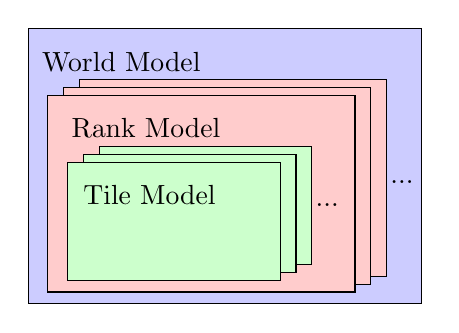
\begin{tikzpicture}
%World Model
\draw [fill=blue!20] (0,1.5) rectangle (5.,5.);
\node[text width=2.25 cm,align=left,below=5pt] at (1.3,5.0) {World Model};
\draw [fill=red!20] (0.65,1.85) rectangle (4.55,4.35);
\draw [fill=red!20] (0.45,1.75) rectangle (4.35,4.25);
\draw [fill=red!20] (0.25,1.65) rectangle (4.15,4.15); %3.5 2.5
\node[text width=0.4 cm] at (4.8, 3.05) {...};
\node[text width=2 cm,align=left,below=5pt] at (1.55,4.15) {Rank Model};
\draw [fill=green!20] (0.9,2.0) rectangle (3.6,3.5);
\draw [fill=green!20] (0.7,1.9) rectangle (3.4,3.4);
\draw [fill=green!20] (0.5,1.8) rectangle (3.2,3.3);
\node[text width=0.4 cm] at (3.85, 2.75) {...};
\node[text width=2 cm, align=left,below=5pt] at (1.7,3.3) {Tile Model};
\end{tikzpicture}
\caption{Each world model is able to aggregate rank models, which aggregate tile models. This allows for representations of the system with various levels of completeness.}
\label{fig:localmodels}
%\vspace{-5mm}
\end{figure}

\subsection{Static load balancing}

%The first attempt at solving the load-balancing problem arises from Seny et al \cite{seny}. 
By re-imagining the wetting and drying algorithm as a type of multirate timestepping, where the dry elements have an infinitely large timestep and the wet elements advance at the implemented timestep, we use the static load balancing approach outlined in \cite{seny}. Here the goal is to assign an equal number of dry elements and wet elements to each rank. This is accomplished by using the multi-constraint graph partitioning outlined in \cite{KKMC}. Note that balancing the memory and load constraints and balancing the wet and dry elements are equivalent formulations of the same load balancing problem.

\subsection{Dynamic load balancing}
Dynamic load balancers in our context are defined as load balancing strategies that operate in an entirely {\em distributed, asynchronous}  manner.
The methods relocate tiles based on a ``load pressure''---the local difference in loads. The idea is to issue many individual relocation requests based on these local observations, and thereby achieve a global balance.

To accommodate both memory and load balance objectives, we implement the refinement procedure used in \cite{KKMC}.
Specifically, our asynchronous diffusion approach includes no world model, but we include tile models and rank models outlined in Listings \ref{lst:tm} and \ref{lst:rm}.


\begin{lstlisting}[
float,
label={lst:tm},
caption={Asynchronous Diffusion Tile Model}]
struct TileModel {
  int my_rank;
  map<int,int> neigh_rank;
  double wet_fraction;  
  double get_gain(int rank);
  void local_broadcast();
};
\end{lstlisting}

\begin{lstlisting}[
float,
label={lst:rm},
caption={Asynchronous Diffusion Rank Model}]
struct RankModel {
  map<int,pair<double,double>> rank_weight;
  StealQ boundary_data;
  void local_broadcast();
  void update_boundary(int leaving);
  void steal_one_tile();
};
\end{lstlisting}

The tile model consists of the tile's wet fraction, the location of neighboring tiles, and a communication gain function, which determines the net impact on inter-rank communication were the tile to be relocated.
The rank model aggregates its tile models to include the tiles bordering the rank, changes in the rank's load balance, and a list of neighboring ranks. These neighboring tiles are stored in the \texttt{StealQ}.
A rank periodically broadcasts its load balancing information to its neighbors,
%Due to the symmetric nature of the communication pattern, 
allowing ranks to aggregate the load state of neighboring ranks.
The execution model does not guarantee message ordering. In order to ensure correctness, both tile and rank models call a \texttt{local\_broadcast} function, which updates neighbors' rank and tile states at regular intervals.
The \texttt{StealQ} contains two STL maps for each rank. This data structure allows us to prioritize, which tile to steal to balance an imbalance in wet or dry tiles from a given rank. The maps are sorted by the amount of extra communication that would be required after stealing a given tile; we prioritize stealing tiles that minimize this additional communication.

During the execution of a task, the tile checks to determine if the wet fraction has switched between wet and dry states.
In the case this happens, the tile's local broadcast updates neighboring tile models.
%, which is then incorporated into the neighbors' rank models.
AGAS {\tt visit} is utilized to ensure that updates are delivered to the tiles no matter where they are located.
The rank model periodically calls \texttt{steal\_one\_tile()}.
Based on the rank model's estimation of the neighboring ranks' work and memory loads, the rank assembles a priority queue $\mathcal{PQ}$ sorted by normalized wet- and dry-element counts.
Only ranks that are overworked or have too many tiles will be inserted into this queue; overburdened ranks will never steal tiles. Karypis and Kumar note this stealing heuristic may lead to chatter, which is when tiles get passed back and forth between the same ranks. To mitigate this, we introduce admissible pressure gradients, i.e. a required minimum imbalance to warrant being inserted into the pool of candidate ranks to be stolen from. Specifically, let the granularity $\mathcal{G}$ be the largest number of elements per tile. For a given rank $r$, let $\mathcal{D}(r)$ be the number of dry elements on rank $r$ and $\mathcal{W}(r)$ the number of wet elements on rank $r$. The precise heuristic for inserting elements is shown in Algorithm \ref{alg:heur}.

\begin{figure}
\begin{algorithm}[H]
\caption{Asynchronous Diffusion Thresholding}
\begin{algorithmic}
\State Set $r$ to current rank ID
\State Set $\Sigma_{\mathcal{W}} \gets \mathcal{W}(r) + \sum_{n \in \text{neighbors}(r)} \mathcal{W}(n)$
\State Set $\Sigma_{\mathcal{D}} \gets \mathcal{D}(r) + \sum_{n \in \text{neighbors}(r)} \mathcal{D}(n)$
\ForAll {$n \in \text{neighbors}(r)$}
    \If {$\mathcal{W}(r) + \alpha \mathcal{G} < \mathcal{W}(n)$}
        \State Insert $n$ into $\mathcal{PQ}(r)$ with weight $\mathcal{W}(n)/\Sigma_{\mathcal{W}}$.
    \EndIf
    \If {$\mathcal{D}(r) + \beta \mathcal{G} < \mathcal{D}(n) $}
        \State Insert $n$ into $\mathcal{PQ}(r)$ with weight $\mathcal{D}(n)/\Sigma_{\mathcal{D}}$.
    \EndIf
\EndFor
\end{algorithmic}
\label{alg:heur}
\end{algorithm}
\end{figure}
Then, we attempt to find the tile on the most imbalanced neighboring rank, which borders the stealing rank and would result in the best communication gain. If there is no satisfactory tile to select, we attempt to improve the most imbalanced constraint associated with the next most-imbalanced rank.

\subsection{Semi-static load balancing}
While the dynamic load balancing procedure allows for fully distributed load balancing decisions, it is unclear that this will result in a good global load balance. The multi-constraint partitioning problem may result in unconnected partitions \cite{KKMC}.  Additionally, the thresholding heuristic is unable to correct gradual--yet large--load imbalances.

To ensure, that we have a good load balance, we consider a semi-static approach which periodically rebalances the global model.  In our formalism, the tile model updates the world model with its wet fraction at a fixed frequency.  Therefore, we can trigger a load balance when all the tiles have sent their information without having to perform any synchronization. %Additionally,
%since we don't begin load balancing until all tile models' messages have been processed, this coordination of broadcast frequency 
%we can minimize the staleness of the tile models by ensuring that all the tiles send their information within a relatively small time interval.
The global model incorporates all the information required to perform load balancing, i.e. the current tile partition and an approximation to the current wet fractions of the respective tiles. The global model is the only entity which may issue {\tt relocate}s, as such the tile partition stored in the global model is always accurate.
%\todo{we removed the more complex algorithm referenced here}

Semistatic rebalancing involves constructing an updated tile-to-rank assignment based on the constraints associated with the updated wet fractions using the multi-constraint graph partitioning algorithm \cite{KKMC}. To keep the master threads available to process messages, we offload the relatively expensive rebalancing operations onto the worker threads where the global model is stored. After obtaining this new partition, we potentially have the means to load balance the system. However, the multi-constraint graph partitioner is unable to take into account the previous location of the tiles. As a worst case scenario, the graph partitioner could return the same partition with permuted partition IDs. The resulting relocation would require migration of every tile, whereas simply maintaining the old partition we would achieve the same load balance without disruption.
In order to remedy this, we solve a minimization problem which determines a permutation in the global rank ID names, which minimizes the number of tiles to be migrated. Using a greedy method, we construct a priority queue of old ID and new ID pairs weighted by the number of tiles that reside in both partitions. We then pop the members of the priority queue until all of the ranks have been assigned new IDs.
This approach can have a significant impact on the number of tiles migrated: for example, during a 1200 core run with 4,400 tiles, the greedy assignment reduced the total number of tiles migrated from roughly 317,000 to 106,000.
\section{Numerical Experiments}
\label{sec:experiments}


\subsection{Empirical Validation of DGSim}
\label{sec:experiments:validation}
\begin{table}
\caption{DGSim parameters for load balance comparison.
%The NUMA domains corresponds NUMA domains per node.
%Worker threads corresponds to worker threads per NUMA domain.
%$R-K$ stages is the total number of Runge-Kutta stages simulated.
%$p$ is the polynomial order of the DG method.
%The rebalance frequency corresponds to the delay between which tiles send messages to the world model. $\alpha$ and $\beta$ are the parameters in the cost model $C(N) = \alpha N/N_{\text{total}} + \beta$.
}
\label{tab:lbc:machine}
\centering
{ \scriptsize
\begin{tabular}{|l|c|l|c|}
\hline
\multicolumn{2}{|c|}{Machine} & \multicolumn{2}{|c|}{DGSWEM} \\
\hline
NUMA domains/node   & 2       & Runge-Kutta Stages     & 273600 \\
Threads/NUMA domain & 12      & Polynomial order ($p$) & 2      \\ 
CPU clock-speed & 2.4 GHz & Tiles/worker thread    & 4      \\
\hline
\multicolumn{2}{|c|}{Asynchronous Diffusion} & \multicolumn{2}{|c|}{Semi-Static} \\
\hline
Rebalance Frequency &  $40\,\mathrm{ms}$  & Rebalance Frequency & $5\,\mathrm{s}$ \\
$\alpha$ & 1 & &  \\
$\beta$ & 2 & & \\
\hline
\end{tabular}
}
\end{table}

To ensure that our simulator is accurate, we compared the DGSim execution times for the Storm36 synthetic hurricane simulation to a skeletonized version of DGSWEM run on NERSC's Edison.  The skeletonized DGSWEM implements the programming model outlined in Section~\ref{sec:dgsim}. Inter-process communication is achieved through one-sided asynchronous remote procedure calls using UPC++~\cite{Bachan2017}, and tasks are executed using a dataflow execution model with a master-worker thread organization.
One feature not implemented in the skeletonized DGSWEM is the AGAS layer. However, for the statically balanced problems considered for this validation, AGAS overhead is negligible due to caching of neighbors' ranks.
By burning identical worker thread execution times, the validation examines whether the messaging and threading overhead models as described in Section~\ref{sec:compute-cost-model} are reasonable.
%, implemented using the programming model described in Section~\ref{sec:dgsim}. 
The parallel efficiencies for the two simulations are shown in Figure~\ref{fig:cal:validation}. Differences in execution times between the simulation and the skeletonized DGSWEM application do not exceed 7\% of the runtime. Furthermore, the DGSim execution time was slower than the DGSWEM execution time for all simulations, reflecting the conservative design of our cost models.  These validation results demonstrate that despite our relatively simple network model, DGSim predicts execution times for this particular hurricane simulation with accuracies comparable to more sophisticated approaches, e.g. \cite{Stanisic2015,Jain2016}.

\begin{figure}
  \centering
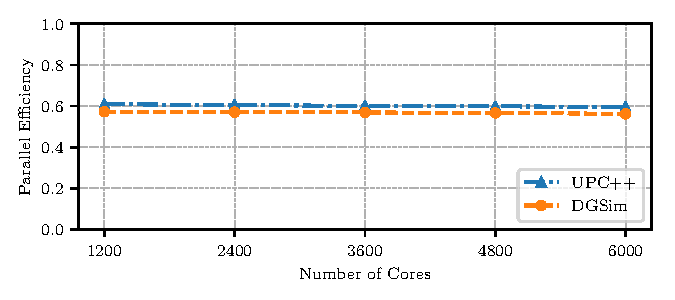
\includegraphics{{load_balancing/images/hurricane_validation_p2}.pdf}
\caption{Comparison between the parallel efficiency of the simulated performance (DGSim) and the skeletonized application code (DGSWEM) on NERSC's Edison supercomputer for 1200 to 6000 cores for the Storm36 hurricane using Machine and DGSWEM parameters as outlined in Table~\ref{tab:lbc:machine}. Each configuration was run five times. The standard deviations for a given core count were each below 1\%.}
\label{fig:cal:validation}
\end{figure}

\subsection{Load Balance Comparison}
In order to compare the load balancing algorithms outlined in Section \ref{sec:balancers}, we compare performance for the hurricane used in the previous subsection using a fixed machine and algorithmic configuration outlined in Table \ref{tab:lbc:machine}. The load balancer parameters are based on parameter sweeps done at 1200 and 3600 cores.

\begin{figure*}
\centering
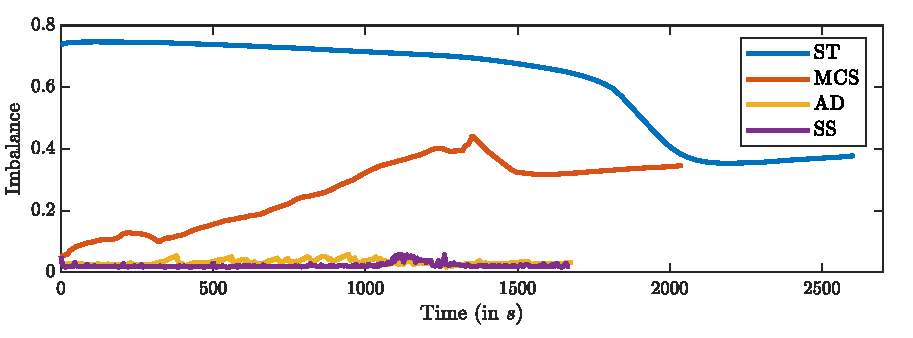
\includegraphics{{load_balancing/images/imbalance}.pdf}
\caption{Load imbalance for Storm 36 using 1200 cores with the configuration outlined in Table \ref{tab:lbc:machine}. The following load balancing strategies were evaluated: static (ST), multi-constraint static (MCS), asynchronous diffusion (AD), and semi-static (SS).}
\label{fig:lbc:imb}
\end{figure*}
%\clearpage
\begin{sidewaystable}
  \centering
  \caption{Performance of load balancers for Storm36}
  \label{tab:sss:res}
	\begin{threeparttable}
	{\footnotesize
	%Generated with make_tables.py
%Do not edit this file directly
%Rather edit make_tables.py
\begin{tabular}{|c||c|c|c|c|c|c|c|c|c|c|c|c|c|}
\hline
& \multicolumn{1}{|c|}{Static} & \multicolumn{2}{|c|}{Multi-constraint static} & \multicolumn{5}{|c|}{Asynchronous diffusion} & \multicolumn{5}{|c|}{Semi-static} \\
\hline
Cores & $T_{\text{ST}}$ & $T_{\text{MC}}$ & $S_{ST}$ & $T_{\text{AD}}$ & TM & $\sigma_{TM}$ & $S_{ST}$ & $S_{MC}$ & $T_{\text{SS}}$ & TM & $\sigma_{TM}$ & $S_{ST}$ & $S_{MC}$ \\
\hline
1200 & 2,613 & 2,048 & 1.28 & 1,686 & 3,654 & 145 & 1.55 & 1.21 & 1,675 & 723,109 & 2,325 & 1.56 & 1.22 \\
\hline
2400 & 1,310 & 1,058 & 1.24 & 849 & 9,532 & 189 & 1.54 & 1.25 & 856 & 681,654 & 557 & 1.53 & 1.24 \\
\hline
3600 & 876 & 698 & 1.26 & 571 & 16,614 & 319 & 1.53 & 1.22 & 585 & 641,950 & 568 & 1.50 & 1.19 \\
\hline
4800 & 659 & 553 & 1.19 & 431 & 24,402 & 319 & 1.53 & 1.28 & 452 & 593,709 & 3,932 & 1.46 & 1.22 \\
\hline
6000 & 528 & 444 & 1.19 & 348 & 36,955 & 761 & 1.52 & 1.28 & 373 & 574,109 & 1,255 & 1.41 & 1.19 \\
\hline
\end{tabular}

	}
	\begin{tablenotes}[para,flushleft]
{\bf Note:} All times are reported in seconds. For each case, 5 runs were performed. The standard deviation of all execution times was found to be below 2\% of the mean. $T$ corresponds to the execution time in seconds. TM refers to the number of relocated tiles. The speed-up $S_X$ is the speed-up of the simulation relative to strategy $X$ at the given core count. Due to non-determinism in our simulation, we've reported standard deviations of tiles moved $\sigma_{TM}$ for a sample size of 5.
\end{tablenotes}
	\end{threeparttable}
\end{sidewaystable}

%\begin{table}[t!]
%\small
%\centering
%\input{images/lb_comparison_table_p2_tpt4}
%\caption{Run-times $T$, in seconds, for the load balancing strategies. The presented speed-ups $S$ are with respect to the static run-time. $TM$ represents the numbers of tiles moved. The non-deterministic nature of the simulation causes variance in the results. We have shown the respective standard deviations $\sigma$ for a sample size of 5. The standard deviations of all the timing data is within 1\%.}
%\label{tab:lbc:speedup}
%\vspace{-7mm}
%\end{table}
%discuss advantage of going to static1

To quantify the quality of our load balancing algorithms, we use two performance metrics: the
\emph{compute intensity}, which is defined for a given rank as the fraction of time spent computing at a given instant in the simulation, and the \emph{imbalance}, which is defined as
\begin{equation*}
I = \frac{ \max T - \overline{T}}{\overline{T}},
\end{equation*}
where $\max T$ is maximum load on a given rank and $\overline{T}$ is the average load across the system. The combined performance results are shown in Figure~\ref{fig:lbc:imb} and the elapsed times and speed-ups in Table \ref{tab:sss:res}.

\begin{figure*}
    \centering
    \subfloat[][Static\label{fig:ci:st}]{
        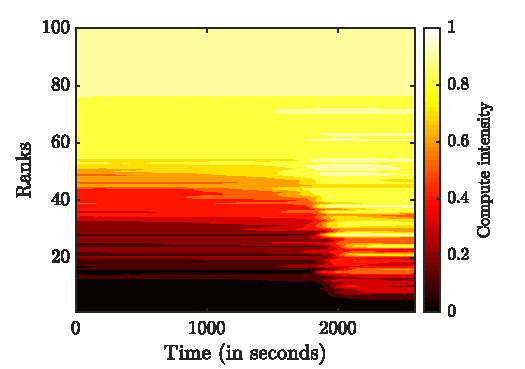
\includegraphics[width=0.44\textwidth]{{load_balancing/images/st_comput_int}.pdf}
    }
\quad
    \subfloat[][Multi-constraint static\label{fig:ci:mcs}]{
        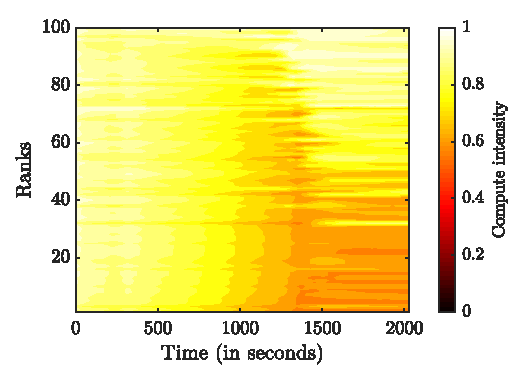
\includegraphics[width=0.44\textwidth]{{load_balancing/images/mcs_comput_int}.pdf}
    }
\\
    \subfloat[][Asynchronous diffusion\label{fig:ci:ad}]{
        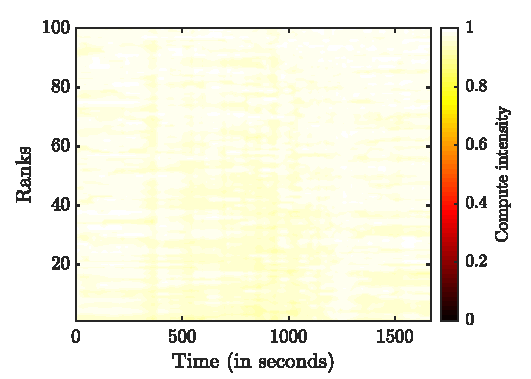
\includegraphics[width=0.44\textwidth]{{load_balancing/images/ad2_comput_int}.pdf}
    }
\quad
    \subfloat[][Semi-static\label{fig:ci:ss}]{
        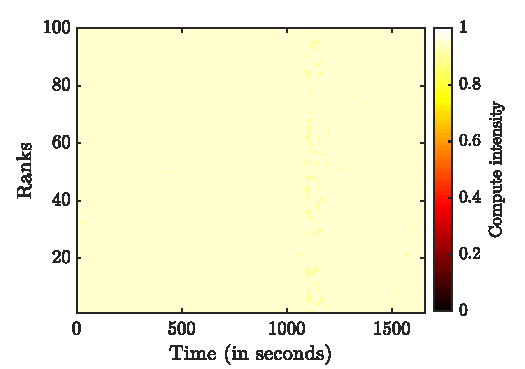
\includegraphics[width=0.44\textwidth]{{load_balancing/images/ss_comput_int}.pdf}
    }
    \caption{Compute intensities of the various load balancing strategies for a 1200 core simulation. For clarity, the ranks have been sorted according to average compute intensity.}
    \label{fig:ci}
\end{figure*}

Since the traditional static load balancing approach solely distributes tiles to ranks to satisfy the memory constraint, it is expected that the static curve in Figure \ref{fig:lbc:imb} has a high imbalance. This is reflected in Figure \ref{fig:ci:st}, where roughly half the ranks are underutilized until the storm inundates the coast. This load profile is consistent with the ~60\% parallel efficiency observed in Figure \ref{fig:cal:validation}.
The multi-constraint static load balancer takes load as well as memory into account. This results in much better load balance until the hurricane makes landfall. Once this happens, the dynamic nature of the computational load causes a strong increase in imbalance and a corresponding decrease in computational intensity. Since the majority of the time DGSWEM simulates is prior to landfall, the multi-constraint static mesh partitioning achieves a speed-up of 1.28 versus the original static partitioning.

Both the asynchronous diffusion and semi-static load balancers are very effective at reducing load imbalance. The compute intensities shown in Figure~\ref{fig:ci:ss} and \ref{fig:ci:ad} illustrate the ranks are being well utilized throughout the simulation. With roughly equal execution times, both load balancers achieve 96\% of the ideal parallel efficiency. 
While the semi-static strategy migrates significantly more tiles than asynchronous diffusion, we have observed a small dependence of execution time in DGSIM on tiles moved.
% We have examined means to reduce the number of times.
AGAS's ability to overlap computation and tile migration minimizes resource starvation. Furthermore, the execution time is mainly determined by the simulation's critical path. Thus migrating tiles not on the critical path will not impact execution time.


\subsection{Strong Scaling Study}
To demonstrate that these algorithms are scalable for operationally-relevant core counts, we present a strong scaling study for up to 6000 cores. 
%Describe simulation
To obtain an understanding of the quality of the load balancers relative to achievable performance, we define the parallel efficiency $E$ for load balancer $LB$ as $E_{LB} = \frac{ T^*}{n_c T_{LB}}$ where $T^*$ is the serial execution time, $n_c$ is the core count, and $T_{LB}$ is the execution time at a given core count. As the master threads do not compute tasks themselves, the best attainable parallel efficiency is 91.7\% = 11/12.

Using the parameters Table \ref{tab:lbc:machine}, the parallel efficiencies for the four partitioning strategies are shown in Figure~\ref{fig:sss:res}. Note that by fixing  tiles per worker thread, the task granularity decreases as we scale out to higher core counts.
Firstly, we note that the code scales well: the static partitioning strategy loses less than 1\% parallel efficiency across the range of core counts. The execution time here should be similar to that of a fully wetted mesh, and demonstrates the parallelizability of the DG method. Next, the multi-constraint static partitioner experiences a slight degradation in performance; $E^{MC}_{6000}/E^{MC}_{1200} = 92.1 \%$. As the number of cores increases each NUMA domain is assigned a smaller fraction of the mesh. Scaling out, the imbalance becomes more sensitive to local inundation, causing degradation of the strong scaling performance.

The semi-static load balancer also loses efficiency at scale with $E^{SS}_{6000}/E^{SS}_{1200}=89.6\%$. Since the rebalance frequency is fixed by the trellis approach, as we scaled out to larger core counts, the number of times the balancer is called decreases. Furthermore, the cost of repartitioning the tile graph increases. \Pingali{At 1200 simulated cores, the METIS calls take approximately $700\,\mathrm{ms}$. These timings increase to around $3700\,\mathrm{ms}$ at 6000 simulated cores.} We suspect that the performance degradation is due to both the faster rate that imbalance is introduced, as well as a mismatch between the load balance used to compute the repartitioning and the load balance at the time when the AGAS migrates get issued. %\todo{See if noburn results help explain things better}
 Ultimately, the performance appears to remain robust, with the semi-static partitioner maintaining a speed-up of 1.19 over the multi-constraint static partitioner at 6000 cores.

The asynchronous diffusion load balancing scales the best with $E^{AD}_{6000}/E^{AD}_{1200} = 96.9\%$. Since the cost of rebalancing is entirely local, the computational complexity of load balancing decisions does not grow with the number of cores. Furthermore, since the rebalancing frequency is roughly two orders of magnitude higher than the semi-static rebalancing frequency, the asynchronous diffusion approach does not struggle with increased irregularity due to higher core counts. A common problem with strong scaling of diffusion-based algorithms is the persistence of small gradients. Even with finer tiles at large core counts, as the rank graph grows, the maximum allowable imbalance grows as well. This did not appear to be a problem here. However, we do not claim that this approach would work equally well for other applications. Ultimately, the asynchronous diffusion worked very well providing a speed-up of 1.28 over the multi-constraint static partitioning strategy at 6000 cores, and achieved 93.7\% of the maximum attainable speed-up.

\begin{figure}
\centering
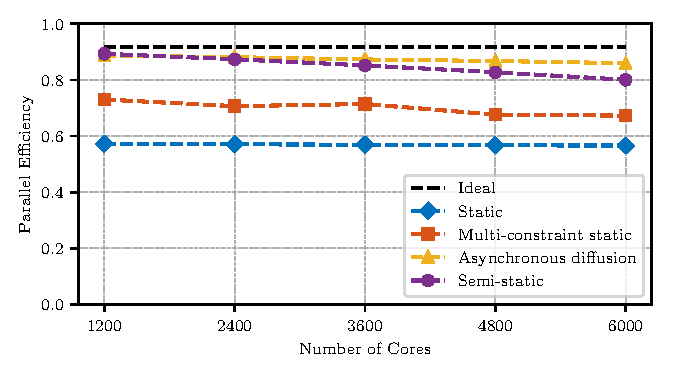
\includegraphics{{load_balancing/images/strong_scaling_p2_tpt4_figure}.pdf}
\caption{Parallel efficiency of the various load balancing strategies on Edison for 1200 to 6000 cores.}
\label{fig:sss:res}
\end{figure}


\section{Conclusion and Future Work}

%\todo[inline]{The impact of future architecture design on the performance of our application is a topic we plan to explore in future work.}

%punchline
Hurricane storm surge simulation stands to benefit greatly from the dynamic load balancing techniques outlined in this paper. 
The irregularity introduced by flooding requires load balancers to simultaneously account for both memory and compute load.
We have presented a dynamic diffusion-based and a semi-static load balancing approach for an asynchronous, task-based implementation of DGSWEM.
To enable rapid prototyping and evaluation of these load balancing strategies, we simulated DGSWEM using a discrete event simulation approach, which
allowed us to evaluate configurations 5,000 times faster than running the actual code (in terms of core-hours).
We found that static multi-constraint partitioning gives a speed-up of 1.28 over static single-constraint balancing. Both semi-static and asynchronous diffusion approaches worked very well, achieving speed-ups of 1.2 over the static multi-constraint partitioning strategy at 1200 cores. The asynchronous diffusion approach scaled best, maintaining a speed-up of 1.52 over the original static partitioning approach at 6000 cores. Furthermore, the asynchronous diffusion approach migrated an order of magnitude fewer tiles than the semi-static approach.

The irregularity of the hurricane limits the need for more sophisticated approaches. By only simulating every tenth timestep, we have exaggerated the rate of change of the imbalance by a factor of ten. In practice, we expect the methods proposed here to completely balance the compute load. Implementing these load balancing strategies in DGSWEM is a topic of future work.

%outline problem
The nature of simulating DGSWEM opens up many interesting avenues of future research.
We plan to model parallel performance behavior of DGSWEM on future supercomputer architectures, e.g. x86 many-core, GPU, and RISC cores.
Additionally, we would like to perform a co-design exploration of algorithmic and software optimizations in conjunction with the hardware parameter space.
Increased communication costs on future architectures will likely play a role in choosing between load balancing strategies that trade between load balance quality, application communication costs, and tile migration costs.
% For example, asynchronous diffusion would have much lower tile migration costs compared to the semi-static approaches at the expense of worse load balance.  SS would have higher tile migration costs compared to SS2, but may have lower application communication costs due to better tile coherence (less shattering).
%\input{load_balancing/acknowledgement}

%\clearpage
%% LaTeX template for Artifact Description appendix used for SC17
% V20170220
%% V20170220
% (C)opyright 2017

% Derived with permission by Michael Heroux (Sandia National Laboratories, St. John's University, MN)
% from ae-20160509.tex 
% written by Grigori Fursin (cTuning foundation, France and dividiti, UK) 
% and Bruce Childers (University of Pittsburgh, USA)
% (C)opyright 2014-2016

\appendix\section{Artifact Description: Adaptive Total Variation Stable Local Timestepping for Conservation Laws}
\label{sec:artifact}

%%%%%%%%%%%%%%%%%%%%%%%%%%%%%%%%%%%%%%%%%%%%%%%%%%%%%%%%%%%%%%%%%%%%%
\subsection{Abstract}

As part of the Association for Computing Machinery's reproducibility initiative, this artifact outlines the details of generating the performance comparison in ``Adaptive Total Variation Stable Local Timestepping for Conservation Laws''.

%%%%%%%%%%%%%%%%%%%%%%%%%%%%%%%%%%%%%%%%%%%%%%%%%%%%%%%%%%%%%%%%%%%%%
\subsection{Description (artifact meta information)}
{\small
\begin{itemize}
  \item {\bf Algorithm: } Finite Volume Code with Adaptive Local Timestepping
  \item {\bf Program: } python, C++14
  \item {\bf Compilation: } GNU C++14 Compiler
%  \item {\bf Transformations: }
%  \item {\bf Binary: }
%  \item {\bf Data set: }
  \item {\bf Operating System: } CentOS Linux release 7.6.1810
  \item {\bf Run-time environment: } Stampede2/Skylake partition
%  \item {\bf Hardware: }
%  \item {\bf Run-time state: }
  \item {\bf Execution: } Parallel/Shared Memory
%  \item {\bf Output: }
  \item {\bf Experiment workflow: } Compile; Preprocess meshes; Run simulation.
%  \item {\bf Experiment customization: }
  \item {\bf Publicly available?: } Yes
\end{itemize}
}

\subsubsection{How software can be obtained}
Software is not yet open-source.

\subsubsection{Software dependencies}
Specific version numbers  of software are provided in Table \ref{tab:version}.

\begin{table}
{
\footnotesize
\caption{Version numbers and git hashes of dependencies}
\label{tab:version}
\begin{center}
\begin{tabular}{|c| c|}
\hline
Software & Stampede2 \\
\hline
\pkg{gcc} & 7.1.0\\
\hline
MPI implementation&  impi/17.0.3 \\
\hline
Devastator & 2c0e160\\
\hline
Python & 3.7.3\\
\hline
\pkg{Gurobi} & 9.0.0\\
\hline
\end{tabular}
\end{center}
}
\end{table}

%%%%%%%%%%%%%%%%%%%%%%%%%%%%%%%%%%%%%%%%%%%%%%%%%%%%%%%%%%%%%%%%%%%%%
\subsection{Installation}
Assuming all dependencies are available, the code uses GNU Makefile to build both versions of the code. The Devastator version of the code can be generated using
\begin{lstlisting}
    make threads=48 problem=XXX ics=YYY
\end{lstlisting}
where equation type \lstinline{problem} may either be set to \lstinline{burgers} or \lstinline{swe}. For solving Burgers' equation, \lstinline{ics} may be set to one of \lstinline{constant}, \lstinline{shockwave}, or \lstinline{rarefaction}, and for solving the shallow water equations, \lstinline{ics} may be set to one of \lstinline{constant}, \lstinline{dambreak}, or \lstinline{carrier-greenspan}.
For the MPI version, the make target is \lstinline{lts-mini-app.mpi}. The problem type and initial conditions can be set using the same \lstinline{problem} and \lstinline{ics} flags used for the Devastator executable.

%%%%%%%%%%%%%%%%%%%%%%%%%%%%%%%%%%%%%%%%%%%%%%%%%%%%%%%%%%%%%%%%%%%%%
\subsection{Experiment workflow}
\begin{table}
{\footnotesize
\caption{Shallow water equations configuration for MPI-Devastator Performance Comparison}
\label{tab:env-vars-perf-comp}
\centering
\input{images/config}
}
\end{table}

The workflow requires setting environment variables including input (\lstinline{lts_input_dir}) and output (\lstinline{lts_output_dir}) folders and the name of the mesh file (\lstinline{lts_mesh_file}). The parameters for the runs in Section~\ref{sec:performance-results} are shown in Table~\ref{tab:env-vars-perf-comp}.
From the root directory, the work flow then requires generating the mesh and mesh splitters as well as any input files,
\begin{lstlisting}
    python scripts/mesh_generator.py,
\end{lstlisting}
generating an actor partition, which is only needed for the Carrier-Greenspan problem,
\begin{lstlisting}
    python scripts/partition_actors.py,
\end{lstlisting}
and running the executable. For the synchronous MPI version, we use TACC's \lstinline{ibrun} launcher.

Lastly, we remark that for the polynomial meshes using an MPI simulation, we generate the mesh using an appropriately set \lstinline{warp_type} environment variable, but then manually overwrite the splitters file using the splitters associated with a uniform warp type.

%%%%%%%%%%%%%%%%%%%%%%%%%%%%%%%%%%%%%%%%%%%%%%%%%%%%%%%%%%%%%%%%%%%%%
\subsection{Evaluation and expected result}
Each simulation run will return the execution time in microseconds to the standard output, and additional output information is written to the output directory.


